In order to investigate the effect of shock-ionisation on the transauroral-line technique of electron density measurement\footnote{The effect of shock-ionisation on the transauroral-line density and reddening diagnostic was investigated in a preliminary fashion by \citet{SpenceThesis}.} \citep{Holt2011}, in Figure\;\ref{fig: tr_grid_shock_modelling: tr_shock_ddd_v_vary} I plot the expected TR([OII]) and TR([SII]) line ratios with the radiation-bounded diagnostic grid for photoionised gas that was previously presented in Section \ref{section: stis_seyferts: tr_diagnostics}, Figure\;\ref{fig: stis_seyferts: tr_ddd} (see also Section \ref{section: xshooter_ic5063: properties_of_outflowing_gas: uvb_vis_analysis_and_results: transauroral_lines}, Figure\;\ref{fig: xshooter_ic5063: tr_grid}). The shock models shown on this grid were taken from the library presented by \citet{Allen2008} (generated with the \textsc{MAPPINGS III} code), and are for solar-composition gas.

First, the effect of varying the shock velocity between 0\;\textless\;$v_\mathrm{shock}$\;\textless\;1000\;km\;s$^{-1}$ with a constant magnetic parameter of $B/\sqrt{n}=2$\;$\mu$G\;cm$^{3/2}$ and pre-shock densities of \mbox{$n=1$, 10, 100, 1000\;cm$^{-3}$} was investigated. Assuming a compression factor of $\sim$100 if the gas cools in pressure equilibrium behind the shock \citep{Sutherland2017, Santoro2018}, these correspond to post-shock densities of \mbox{$n=10^2$, 10$^3$, 10$^4$, 10$^5$\;cm$^{-3}$}. From Figure\;\ref{fig: tr_grid_shock_modelling: tr_shock_ddd_v_vary}, it can be seen that for high shock velocities ($\gtrapprox$\;500\;km\;s$^{-1}$) at a given density, the modelled line ratios are similar to those predicted by photoionisation modelling. However, for lower shock velocities (a few hundred km\;s$^{-1}$), the predicted densities may differ by $\pm0.22$ orders of magnitude. Similarly, shock-ionisation may affect the derived colour excesses by $\mathrm{E(B-V)}_\mathrm{TR}\pm0.13$.

Secondly, I investigate the effect of varying the magnetic parameter between typical values for the ISM (2\;\textless\;$B/\sqrt{n}$\;\textless\;4\;$\mu$G\;cm$^{3/2}$: \citealt{Dopita1995, Allen2008}). This was done for three values of shock velocity \mbox{($v_\mathrm{shock}=400, 600, 800$\;km\;s$^{-1}$)}, which is shown in Figure\;\ref{fig: tr_grid_shock_modelling: tr_shock_ddd_bn_vary}. The impact on derived electron densities is greater at higher densities ($\pm0.25$ orders of magnitude) than at lower densities ($\pm0.10$ orders of magnitude), with little effect on the derived reddening value.

Finally, I quantify the effect of simultaneously varying the velocity (between 0\;\textless\;$v_\mathrm{shock}$\;\textless\;1000\;km\;s$^{-1}$) and the magnetic parameter \mbox{(2\;\textless\;$B/\sqrt{n}$\;\textless\;4\;$\mu$G\;cm$^{3/2}$)} on the TR-derived electron densities and reddenings (Figure\;\ref{fig: tr_grid_shock_modelling: tr_shock_ddd_v_bn_vary}). It is found that the effect on the derived density is $\pm0.38$ orders of magnitude, regardless of the density of the modelled gas, and that the effect on derived reddening values is the same as varying the velocity ($\mathrm{E(B-V)}\pm0.13$).

\begin{figure}
    \centering
    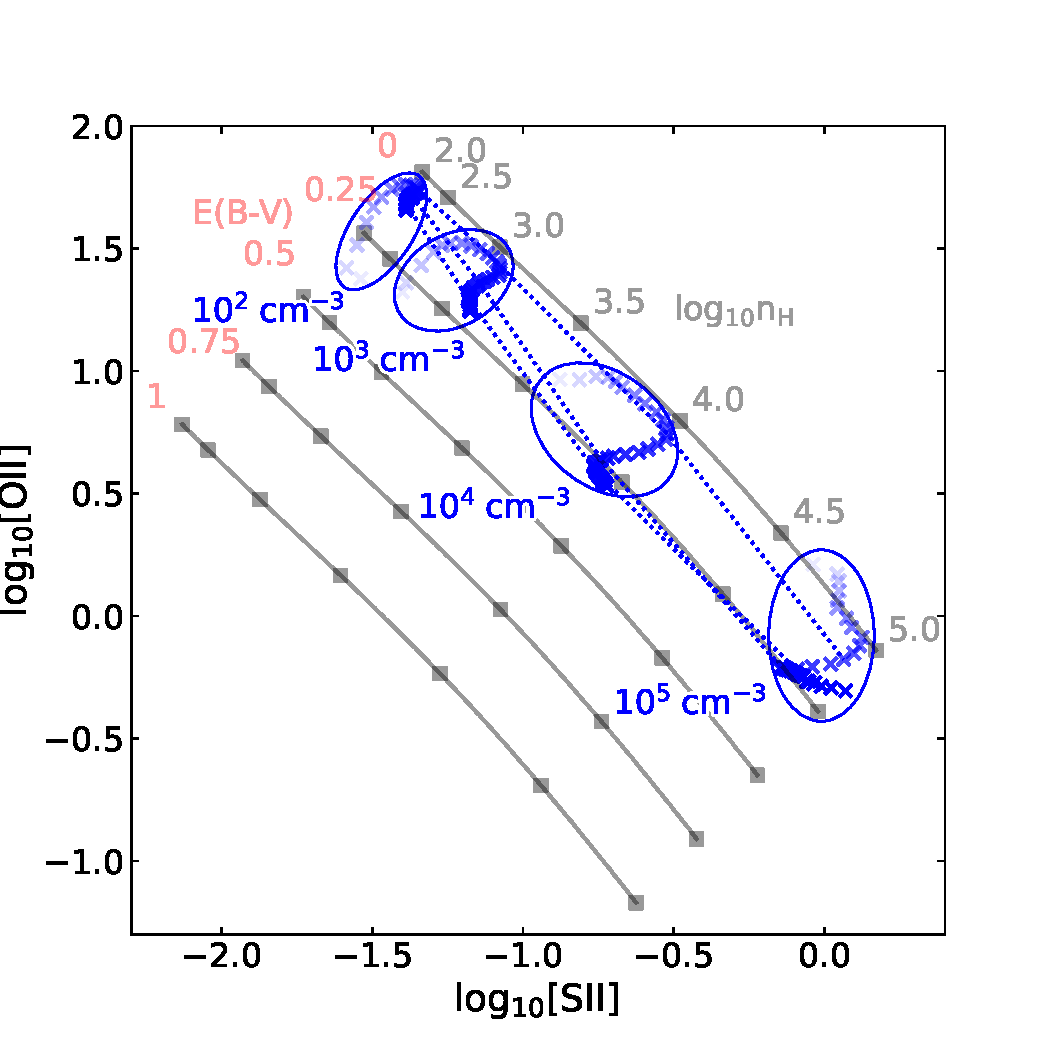
\includegraphics[width=\linewidth]{figures/tr_grid_shock_modelling/tr_shock_ddd_bn2.pdf}
    \caption[Transauroral-line-ratio grid for shock models at a fixed magnetic parameter and a range of shock velocities.]{Transauroral-line-ratio (TR([SII]) vs TR([OII]) grid for radiation-bounded AGN-photoionised gas (black with red E(B-V) labels; as in Figures \ref{fig: xshooter_ic5063: tr_grid} and  \ref{fig: stis_seyferts: tr_ddd}) with the line ratios expected from modelled shocks (blue crosses) of fixed magnetic parameter ($B/\sqrt{n}=2$\;$\mu$G\;cm$^{3/2}$) at different post-shock densities (labelled in blue), and for a range of shock velocities (0\;\textless\;$v_\mathrm{shock}$\;\textless\;1000\;km\;s$^{-1}$). Line ratios from shock modelling at a single post-shock density (assuming a compression factor of 100) are grouped by blue ellipses, and points of the same shock velocity (v$_\mathrm{shock}=400,600,800$\;km\;s$^{-1}$) are joined by dashed blue lines.}
    \label{fig: tr_grid_shock_modelling: tr_shock_ddd_v_vary}
\end{figure}

\begin{figure}
    \centering 
    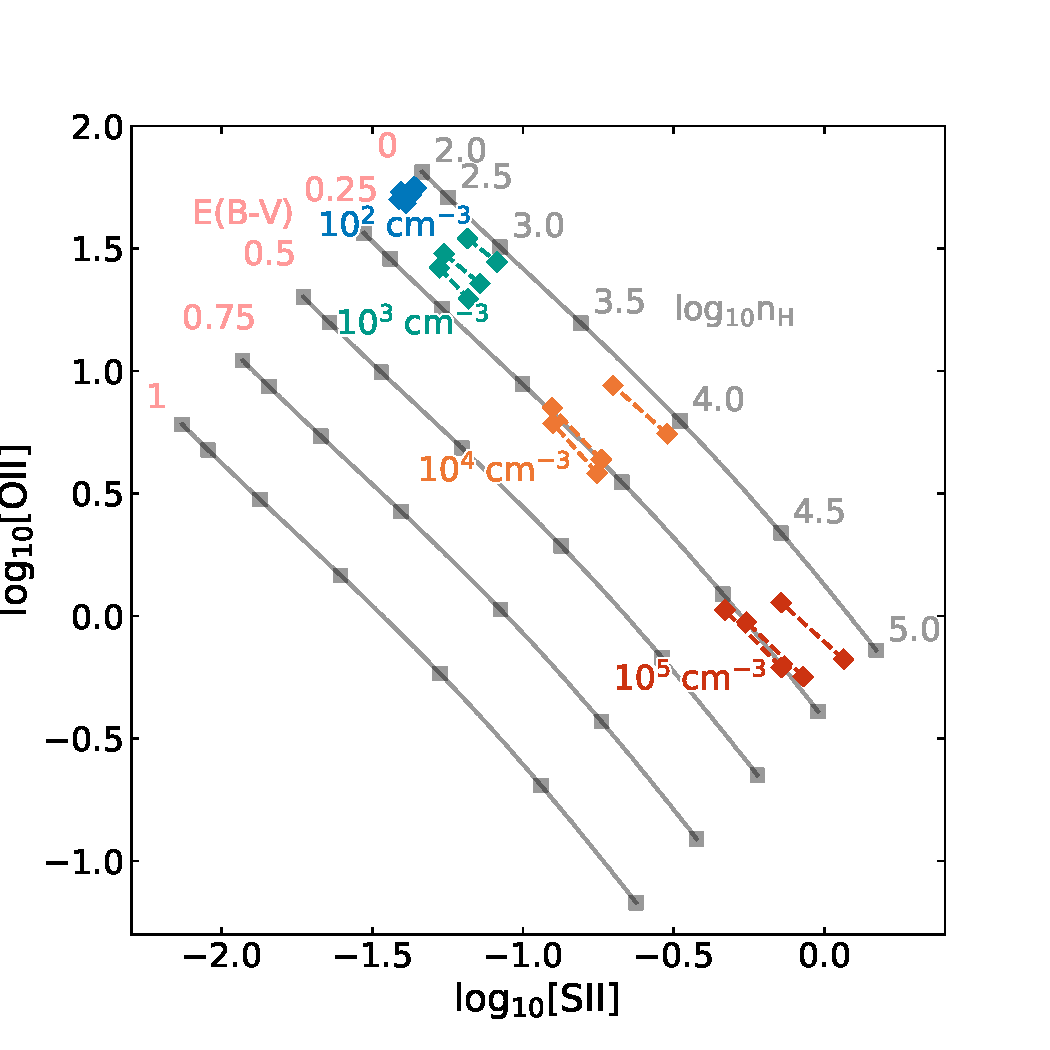
\includegraphics[width=\linewidth]{figures/tr_grid_shock_modelling/tr_shocks_ddd_bn2_bn4.pdf}
    \caption[Transauroral-line-ratio grid for shock models of different magnetic parameters and shock velocities.]{Transauroral-line-ratio grid (as in Figure\;\ref{fig: stis_seyferts: tr_ddd}) with line ratios predicted by shock modelling for three values of shock velocity ($v_\mathrm{shock}=400, 600$ and 800\;km\;s$^{-1}$) and two values of magnetic parameter (2\;\textless\;$B/\sqrt{n}$\;\textless\;4\;$\mu$G\;cm$^{3/2}$) which are typical of the ISM. Line ratios generated using the same post-shock density are shown as crosses with the same colour (labelled), and points of the same density and velocity are joined by a dashed line.}
    \label{fig: tr_grid_shock_modelling: tr_shock_ddd_bn_vary}
\end{figure}

\begin{figure}
    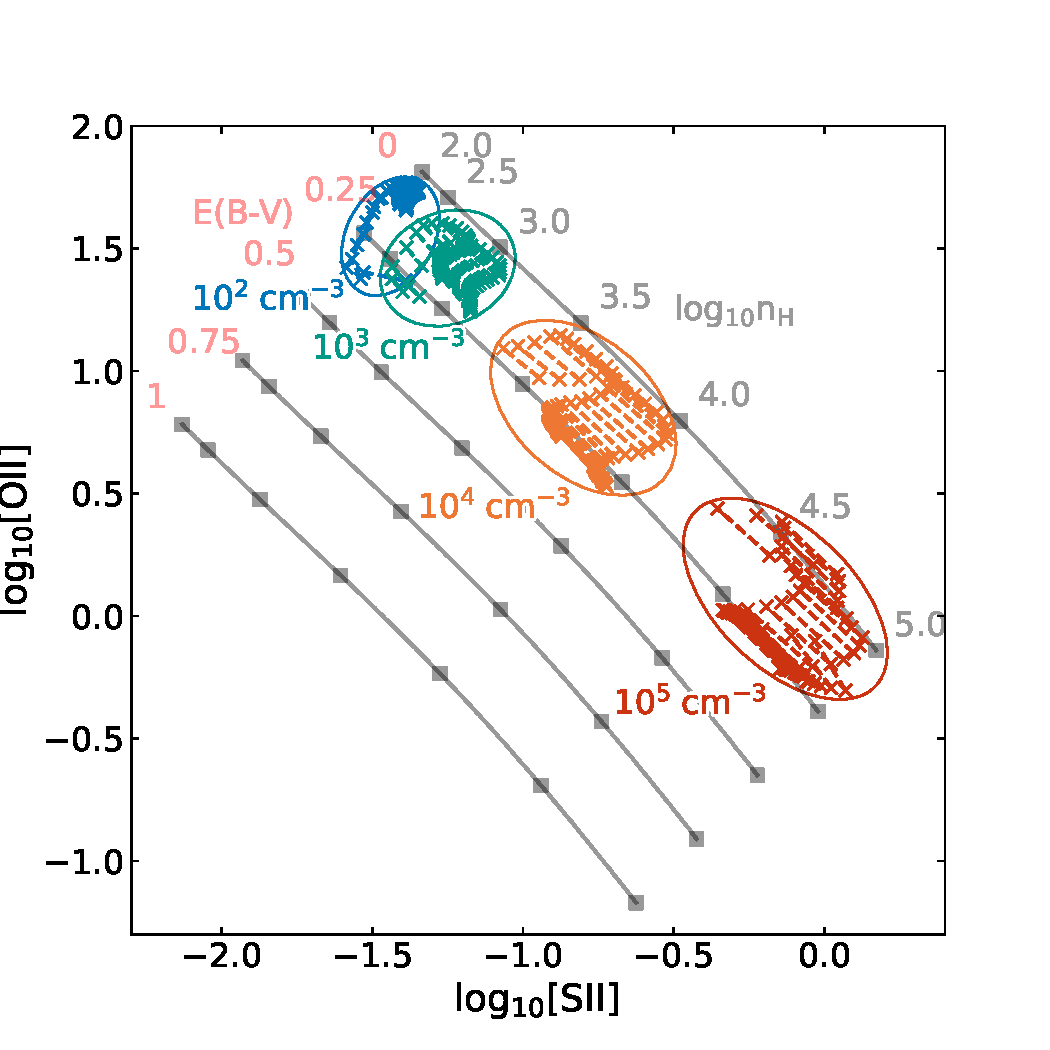
\includegraphics[width=\linewidth]{figures/tr_grid_shock_modelling/tr_shocks_ddd_v_bn2_bn4.pdf}
    \caption[Transauroral-line-ratio grid for shock models of varying magnetic parameters and a range of shock velocities.]{Transauroral-line-ratio grid (as in Figure\;\ref{fig: stis_seyferts: tr_ddd}) with line ratios predicted by shock modelling for two magnetic parameters ($B/\sqrt{n}=2,4$\;$\mu$G\;cm$^{3/2}$) and a range of shock velocities (0\;\textless\;$v_\mathrm{shock}$\;\textless\;1000\;km\;s$^{-1}$) at each value of post-shock density. Predicted ratios with the same post-shock density are shown with crosses of a single colour for each density (labelled) and are grouped with ellipses.}
    \label{fig: tr_grid_shock_modelling: tr_shock_ddd_v_bn_vary}
\end{figure}